\chapter{Теория}
\label{ch:intro}

\section*{\textbf{Введение}}

На прошлом занятии мы познакомились с преобразованием Фурье - инструментом, позволяющим получить спектральную функцию непереодического сигнала.
На этом занятии рассмотрим свойства преобразования Фурье.

\section*{\textbf{Свойство линейности}}

Данное свойство говорит о том, что преобразование Фурье - линейный оператор, т.е он сохраняет линейные комбинации функции. Для нас
это значит, что при сложении сигналов со спектром итогового сигнала не произойдет ничего страшного. Итоговый спектр будет
являться суммой спектров каждого отдельного сигнала. Это также верно и для операции умножения. Все это работает и в обратную сторону. Если мы просуммируем спектры
и выполним ОПФ, то получим сумму сигналов.

$$X(t)\overset{\text{FT}}{\leftrightarrow}X(iw)$$
$$Y(t)\overset{\text{FT}}{\leftrightarrow}Y(iw)$$

$$\alpha X(t) + \beta Y(t)\overset{\text{FT}}{\leftrightarrow}\alpha X(iw) + \beta Y(iw)$$

\subsection*{\textbf{Доказательство}}

Подставим линейную комбинацию напрямую в ПФ:

$$\alpha X(t) + \beta Y(t)\overset{\text{FT}}{\to} \int_{-\infty}^{\infty}[\alpha X(t) + \beta Y(t)]e^{i\omega t}dt$$

Применим свойство интеграла "Интеграл суммы равен сумме интегралов":

$$\alpha X(t) + \beta Y(t)\overset{\text{FT}}{\to} \int_{-\infty}^{\infty}\alpha X(t)e^{i\omega t}dt + \int_{-\infty}^{\infty}\beta Y(t)e^{i\omega t}dt$$

Каждый интеграл и будет результатом ПФ, т.е

$$\alpha X(t) + \beta Y(t)\overset{\text{FT}}{\to} \alpha X(iw) + \beta Y(iw)$$

\section*{\textbf{Свойство смещения или задержки по времени}}

Данное свойство говорит о том, что при сдвиге сигнала во времени на $\tau$, спектр умножится на $e^{-j\omega \tau}$. Это свойство
работает и в обратную сторону, т.е если нам нужно сдвинуть сигнал во времени на $\tau$, мы можем спектр умножить на $e^{-j\omega \tau}$.

$$X(t)\leftrightarrow X(i\omega)$$
$$X(t-\tau_0)\leftrightarrow X(i\omega)e^{-i\omega \tau_0}$$

Временной сдвиг сигнала не меняет форму амплитудного спектра, а меняет только форму фазового спектра.

\subsection*{\textbf{Доказательство}}

Подставим $t-\tau_0$ напрямую в ПФ:

$$X(t-\tau_0) = \int_{-\infty}^{\infty}X(t-\tau_0)e^{-i\omega(t)}dt$$

Пусть $T = t-\tau_0$, тогда выполним замену переменной: $t = T + \tau_0$ и $dt = dT$.

$$\int_{-\infty}^{\infty}X(T)e^{-i\omega(T+\tau_0)}dT = e^{-i\omega \tau_0} \int_{-\infty}^{\infty}X(T)e^{-i\omega T}dT = $$

$$X(i\omega) e^{-i\omega \tau_0} $$

\section*{\textbf{Свойство смещения по частоте (модуляции)}}

Данное свойство говорит о том, что если умножить сигнал на $e^{i\omega_0t}$, то спектр этого сигнала сдвинется в область высоких частот на $\omega_0$.
Причем здесь модуляция? Модуляция это перенос низкочастотного сигнала на высокочастотный сигнал и это свойство как раз помогает сдвинуть
сигнал на высокие частоты, т.е промодулировать его. 

$$X(t)\overset{\text{FT}}{\leftrightarrow}X(i\omega)$$

$$X(t)e^{i\omega_0t}\overset{\text{FT}}{\leftrightarrow} X(i(\omega - \omega_0))$$


\subsection*{\textbf{Доказательство}}

Подставим $e^{i\omega_0t}$ напрямую в ПФ:

$$X(t)e^{i\omega_0t} = \int_{-\infty}^{\infty}e^{i\omega_0t}X(t)e^{-i\omega t} = $$ 

Объединим экспоненты

$$\int_{-\infty}^{\infty}X(t)e^{-i\omega t + i\omega_0t} = \int_{-\infty}^{\infty}X(t)e^{-it(\omega - \omega_0)} = X(i(\omega - \omega_0))$$

\section*{\textbf{Свойство временного масштабирования}}

Это свойство говорит о том, что растяжение/сужение сигнала во времени приводит к сужение/растяжению частотного спектра.
|a| > 1 - сжатие сигнала, |a| < 1 - растяжение сигнала. Коэффициент $\frac{1}{|a|}$ нужен для сохранения энергии сигнала. Это как с
прямоугольным сигналом: если увеличиваем длительность $\tau$ (домножаем на $|a| > 1$), то спектр расширяется, а если уменьшать $\tau$
(домножаем на $|a| < 1$), то спектр сужается. 

$$X(t)\leftrightarrow X(i\omega)$$
$$X(at)\leftrightarrow \frac{1}{|a|}X(\frac{i\omega}{a})$$

\subsection*{\textbf{Доказательство}}

Запишем ПФ над $X(at)$

$$X(at) = \int_{-\infty}^{\infty} X(at)e^{-i\omega t}dt$$

Пусть $T = at \to t = \frac{T}{a}, dt = \frac{dT}{a}$, тогда

$$\int_{-\infty}^{\infty} X(T)e^{-i\omega \frac{T}{a}}\frac{dT}{a} = \frac{1}{|a|}\int_{-\infty}^{\infty} X(T)e^{-iT \frac{\omega}{a}}dT =
\frac{1}{|a|}X(\frac{i\omega}{a})$$

\section*{\textbf{Свойство свертки}}

$$X(t)*y(t) = \int_{-\infty}^{\infty}X(\tau)y(t-\tau)d\tau$$
$$X(t)*y(t) \overset{\text{FT}}{\leftrightarrow} X(i\omega) * y(i\omega)$$
$$X(t)*y(t) \overset{\text{FT}}{\leftrightarrow} \int_{-\infty}^{\infty}X(i\lambda) y(i(\omega - \lambda))d\lambda$$


\section*{\textbf{Связь между длительностью сигнала и спектром}}

Если T - длительность сигнала, W - ширина спектра, то T * W = k * 1

\section*{\textbf{ПФ для прямоугольного видеоимпульса}}

$$S(i\omega) = \int_{-\infty}^{\infty}S(t)*e^{-i\omega t} = \int_{-\frac{\tau}{2}}^{\frac{\tau}{2}}U*e^{-i\omega t} = $$

$$U * \frac{1}{-i\omega t}e^{i\omega t}\bigg|_{-\frac{\tau}{2}}^{\frac{\tau}{2}} = U\frac{1}{-i\omega}[e^{-i\omega\frac{\tau}{2}} - e^{i\omega\frac{\tau}{2}}]$$

В [] видим sin. Умножим выражение на $\frac{\tau}{\tau}$

$$\boxed{U\tau * \frac{sin(\frac{\omega t}{2})}{\frac{\omega t}{2}}}$$

Спектр данной функции будет следующим:

\begin{figure}[H]
    \centering
    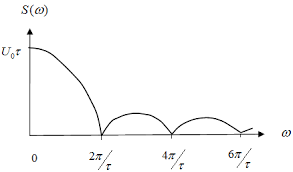
\includegraphics[width=1.0\textwidth]{rect_spec.png}
    \caption{Спектр прямоугольного видеоимпульса}
\end{figure}

Найдем точки, в которых спектральная функция будет обращаться в ноль. Если посомотреть на функцию выше, то можно заметить, что функция
обращается в ноль только при $sin(\frac{\omega t}{2}) = 0$, т.е когда $\frac{\omega t}{2} = \pi n \to \omega = \frac{2\pi n}{\tau}$


\section*{\textbf{ПФ для прямоугольного несимметричного сигнала}}

Прямоугольный несимметричный сигнал отличается от предыдущего сдвигом на $\frac{\tau}{2}$. Формула выводится аналогично, но 
пределы интегрирования будут $[0;\tau]$.

$$\boxed{U\tau * \frac{sin(\omega t)}{\omega t}}$$

\section*{\textbf{Изменение спектра при умножении сигналов разной формы}}

Допустим, мы перемножили прямоугольный сигнал и обычный косинус. Какой спектр при этом получится? Спектр будет похож на нечто
среднее между спектрами исходных сигналов.

\begin{figure}[H]
    \centering
    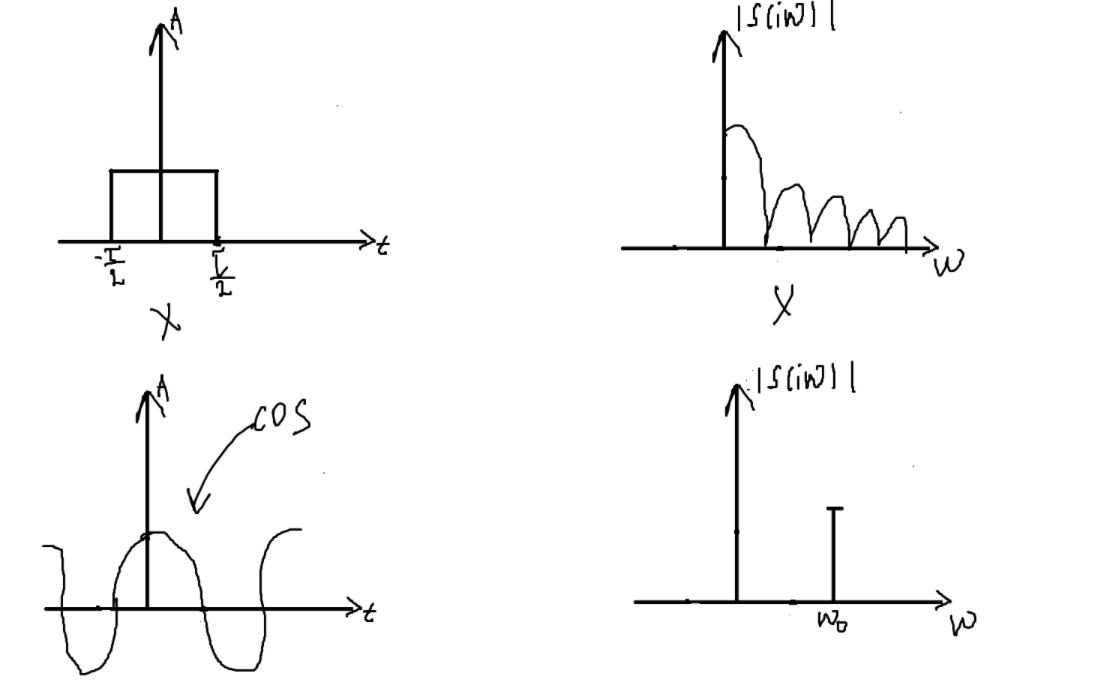
\includegraphics[width=1.0\textwidth]{mul.png}
    \caption{Сигналы разной формы и их спектральные функции}
\end{figure}

\begin{figure}[H]
    \centering
    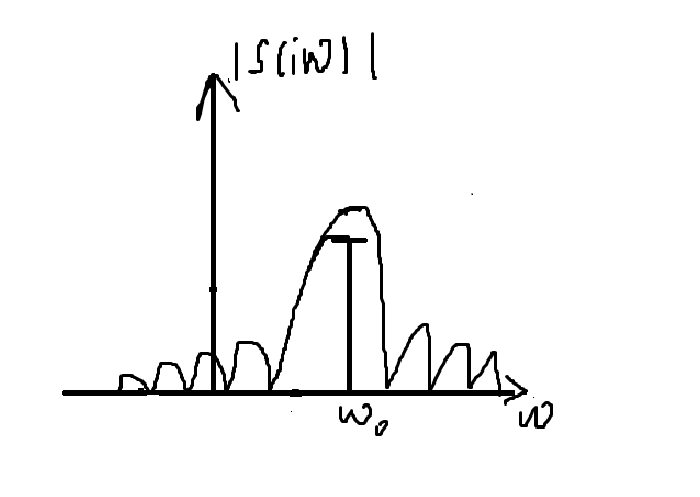
\includegraphics[width=1.0\textwidth]{mul_res.png}
    \caption{Спектральная функция после перемножения}
\end{figure}

Можем видеть, что спектральная функция прямоугольного сигнала как-бы сместилась на частоту $\omega_0$. Такое перемножение сигналов
может происходить при формировании сигнала, если формирующий фильтр имеет прямоугольную импульсную характеристику.

\endinput